\documentclass[10pt,twocolumn]{article}

% ============================================================
% PAKET
% ============================================================
\usepackage[a4paper,left=1.9cm,right=1.9cm,top=2.6cm,bottom=2.2cm,columnsep=0.6cm]{geometry}
\usepackage[T1]{fontenc}
\usepackage[utf8]{inputenc}
% Times New Roman: mathptmx memberikan tampilan setara Times New Roman
% (Times/Nimbus Roman) yang kompatibel dengan pdfLaTeX tanpa memerlukan
% font proprietary terpasang di sistem. Jika ingin font Times New Roman
% asli (.ttf bawaan Windows/Office), kompilasi dengan XeLaTeX/LuaLaTeX
% dan ganti baris ini dengan: \usepackage{fontspec}\setmainfont{Times New Roman}
\usepackage{mathptmx}
\usepackage{amsmath,amssymb}
\usepackage{graphicx}
\usepackage{booktabs}
\usepackage{multirow}
\usepackage{caption}
\usepackage{stfloats}
\usepackage{enumitem}
\usepackage{fancyhdr}
\usepackage{titlesec}
\usepackage{balance}
\usepackage{placeins}
\usepackage{xcolor}
\usepackage{float}
\usepackage[hidelinks]{hyperref}

\captionsetup{font=footnotesize,labelfont=bf,skip=4pt}
\setlength{\parindent}{0pt}
\setlength{\parskip}{0pt}
\setlength{\dbltextfloatsep}{8pt}
\setlength{\textfloatsep}{8pt}
\setlength{\intextsep}{6pt}
\renewcommand{\dbltopfraction}{0.95}
\renewcommand{\dblfloatpagefraction}{0.85}
\renewcommand{\topfraction}{0.95}
\renewcommand{\textfraction}{0.05}

% ============================================================
% FORMAT JUDUL BAGIAN (gaya prosiding: I., II., ... / A., B., ...)
% ============================================================
\titleformat{\section}{\centering\normalfont\fontsize{11}{13}\bfseries}{\Roman{section}.}{0.5em}{}
\titlespacing*{\section}{0pt}{*1.6}{*1}
\titleformat{\subsection}{\normalfont\fontsize{10}{12}\bfseries}{\Alph{subsection}.}{0.5em}{}
\titlespacing*{\subsection}{0pt}{*1.1}{*0.6}

% ============================================================
% HEADER BERJALAN (meniru format prosiding HIMATEKTRO ITS)
% ============================================================
\pagestyle{fancy}
\fancyhf{}
\renewcommand{\headrulewidth}{0.4pt}
\fancyhead[L]{\footnotesize PROSIDING SEMINAR TUGAS AKHIR (2026)\\
\footnotesize Departemen Teknik Elektro\\
\footnotesize HIMATEKTRO ITS}
\setlength{\headheight}{34pt}

% ============================================================
% DOKUMEN
% ============================================================
\begin{document}

\twocolumn[
  \begin{center}
    {\fontsize{15}{18}\selectfont\bfseries Navigasi Robot Beroda Otonom Berbasis Logika Fuzzy\\
    dengan Fusi Sensor LiDAR dan Kamera Termal}

    \vspace{3mm}
    {\fontsize{11}{13}\selectfont Priagung Ramadhan Alfalakhi, Djoko Purwanto, Muhammad Qomaruz Zaman}

    \vspace{1.5mm}
    {\fontsize{9}{11}\selectfont\itshape
    Departemen Teknik Elektro, Fakultas Teknologi Elektro dan Informatika Cerdas,
    Institut Teknologi Sepuluh Nopember (ITS)\\
    Jl. Arief Rahman Hakim, Surabaya 60111\\
    e-mail: 5022221161@student.its.ac.id}
  \end{center}
  \vspace{4mm}
]

\noindent\textit{Abstrak}— Navigasi yang aman merupakan aspek penting pada robot bergerak otonom, terutama ketika beroperasi pada lingkungan \textit{indoor} yang mengandung \textit{obstacle} statis maupun dinamis. LiDAR dua dimensi (LiDAR 2D) yang umum digunakan sebagai sensor utama navigasi memiliki keterbatasan berupa \textit{blind-spot} vertikal, sehingga \textit{obstacle} berprofil rendah berpotensi tidak terdeteksi dan meningkatkan risiko tabrakan. Penelitian ini mengusulkan sistem navigasi robot beroda otonom yang mengintegrasikan LiDAR 2D dan kamera termal melalui pendekatan \textit{decision-level fusion} untuk menghasilkan nilai \textit{effective traversability}, yang selanjutnya digunakan sebagai masukan pengendali fuzzy Mamdani guna menyesuaikan parameter \textit{speed scale} dan \textit{repulsive gain} pada \textit{Artificial Potential Field} (APF) secara adaptif. Sistem diimplementasikan pada ROS Noetic dan diintegrasikan dengan ROS Navigation Stack (NavfnROS sebagai \textit{global planner} dan APFPlanner sebagai \textit{local planner}), kemudian diuji pada simulator Gazebo menggunakan delapan skenario yang meliputi lingkungan terbuka, \textit{obstacle} statis, \textit{obstacle} berprofil rendah pada area \textit{blind-spot} LiDAR, dan \textit{obstacle} dinamis. Hasil pengujian menunjukkan bahwa konfigurasi fuzzy mempertahankan \textit{Success Rate} dan \textit{Collision-Free Rate} sebesar 100\% pada seluruh skenario, sedangkan konfigurasi \textit{baseline} menurun hingga 0\% pada skenario \textit{obstacle} dinamis. Nilai \textit{minimum clearance} juga meningkat signifikan, dari $-0{,}1635$~m (\textit{baseline}, mengalami tabrakan) menjadi $0{,}3167$~m (fuzzy) pada skenario \textit{obstacle} dinamis (uji Mann--Whitney $U$, $p<0{,}001$, $r=1{,}00$). Meskipun menghasilkan penambahan waktu tempuh dan panjang lintasan, metode yang diusulkan mampu mempertahankan margin keselamatan yang jauh lebih besar terhadap \textit{obstacle} selama navigasi berlangsung.

\noindent\textit{Kata Kunci}— robot bergerak otonom, LiDAR 2D, kamera termal, fusi sensor, logika fuzzy Mamdani, \textit{Artificial Potential Field}, ROS Navigation Stack.

\vspace{2mm}

\section{PENDAHULUAN}

Perkembangan robot bergerak otonom (\textit{autonomous mobile robot}) meningkat pesat seiring kebutuhan otomatisasi pada sektor industri, logistik, dan layanan publik. Kemampuan robot bergerak secara mandiri sangat bergantung pada sistem navigasi yang mampu memahami kondisi lingkungan, merencanakan lintasan, dan menghindari \textit{obstacle} secara aman \cite{Liu2024,Macenski2022}.

Pada lingkungan \textit{indoor}, LiDAR dua dimensi banyak digunakan sebagai sensor navigasi utama karena memberikan informasi jarak dengan akurasi tinggi serta kebutuhan komputasi yang relatif rendah, dan telah terintegrasi luas pada sistem berbasis Robot Operating System (ROS) \cite{Macenski2022}. Akan tetapi, LiDAR 2D hanya memindai satu bidang horizontal sehingga \textit{obstacle} yang seluruh profilnya berada di luar bidang tersebut berpotensi tidak terdeteksi \cite{Fagundes2024}. Keterbatasan ini dikenal sebagai \textit{blind-spot} vertikal dan menjadi masalah serius pada lingkungan \textit{indoor} yang sering mengandung \textit{obstacle} berprofil rendah, seperti hewan peliharaan atau benda kecil di lantai \cite{Kibii2022,Fagundes2024}.

Kamera termal berpotensi melengkapi keterbatasan tersebut karena mampu merekam distribusi temperatur objek tanpa bergantung pada karakteristik visual sebagaimana kamera RGB \cite{Castro2016}. Beberapa penelitian menunjukkan bahwa integrasi kamera termal dan LiDAR mampu meningkatkan kualitas persepsi lingkungan karena kedua sensor memiliki karakteristik pengamatan yang saling melengkapi \cite{Choi2023,Schichler2025}. Meskipun demikian, persepsi yang lebih lengkap tetap memerlukan mekanisme pengambilan keputusan yang adaptif. \textit{Artificial Potential Field} (APF) banyak digunakan sebagai metode navigasi reaktif karena formulasinya sederhana dan responsif secara \textit{real-time} \cite{Khatib1986}, namun parameter APF yang bersifat tetap membuat respons navigasi kurang adaptif terhadap perubahan tingkat risiko lingkungan \cite{Lv2024}. Logika fuzzy telah dilaporkan mampu mengatasi keterbatasan tersebut dengan menghasilkan keputusan yang lebih fleksibel tanpa memerlukan model matematis yang kompleks \cite{Haider2022,Benaicha2026}.

Berdasarkan permasalahan tersebut, penelitian ini mengusulkan sistem navigasi robot beroda otonom yang mengintegrasikan LiDAR 2D dan kamera termal melalui fusi \textit{traversability} pada tingkat keputusan (\textit{decision-level fusion}), kemudian memanfaatkan logika fuzzy Mamdani sebagai lapisan adaptif yang menyesuaikan parameter \textit{speed scale} dan \textit{repulsive gain} pada APF berdasarkan kondisi lingkungan yang diamati. Sistem dibangun di atas ROS Navigation Stack tanpa mengubah struktur dasarnya, dan dievaluasi pada simulator Gazebo menggunakan delapan skenario pengujian yang mencakup lingkungan terbuka, \textit{obstacle} statis, \textit{obstacle} berprofil rendah pada area \textit{blind-spot} LiDAR, serta \textit{obstacle} dinamis. Makalah ini disusun sebagai berikut: Bagian II memaparkan metodologi perancangan sistem, Bagian III menyajikan hasil pengujian beserta pembahasannya, dan Bagian IV memuat kesimpulan penelitian.

\section{METODOLOGI PENELITIAN}

\subsection{Arsitektur Sistem}

Sistem navigasi dibangun secara modular berbasis ROS s\-ehingga setiap fungsi direalisasikan sebagai \textit{node} yang saling bertukar data melalui mekanisme \textit{publish--subscribe} \cite{Macenski2022}. Arsitektur keseluruhan terdiri atas dua jalur persep\-si yang berjalan paralel, yaitu jalur kamera termal da\-n jalur LiDAR, yang masing-masing menghasilkan skor \textit{traversability}. Kedua skor digabungkan pada tahap fusi untuk menghasilkan \textit{effective traversability} yang menjadi salah satu masukan pengendali fuzzy Mamdani. Keluaran fuzzy kemudian memodifikasi parameter \textit{local planner} berbasis APF sebelum perintah kecepatan diterbitkan ke robot. Gambar~\ref{fig:arsitektur} menunjukkan arsitektur lengkap sistem.

\begin{figure*}[t]
\centering
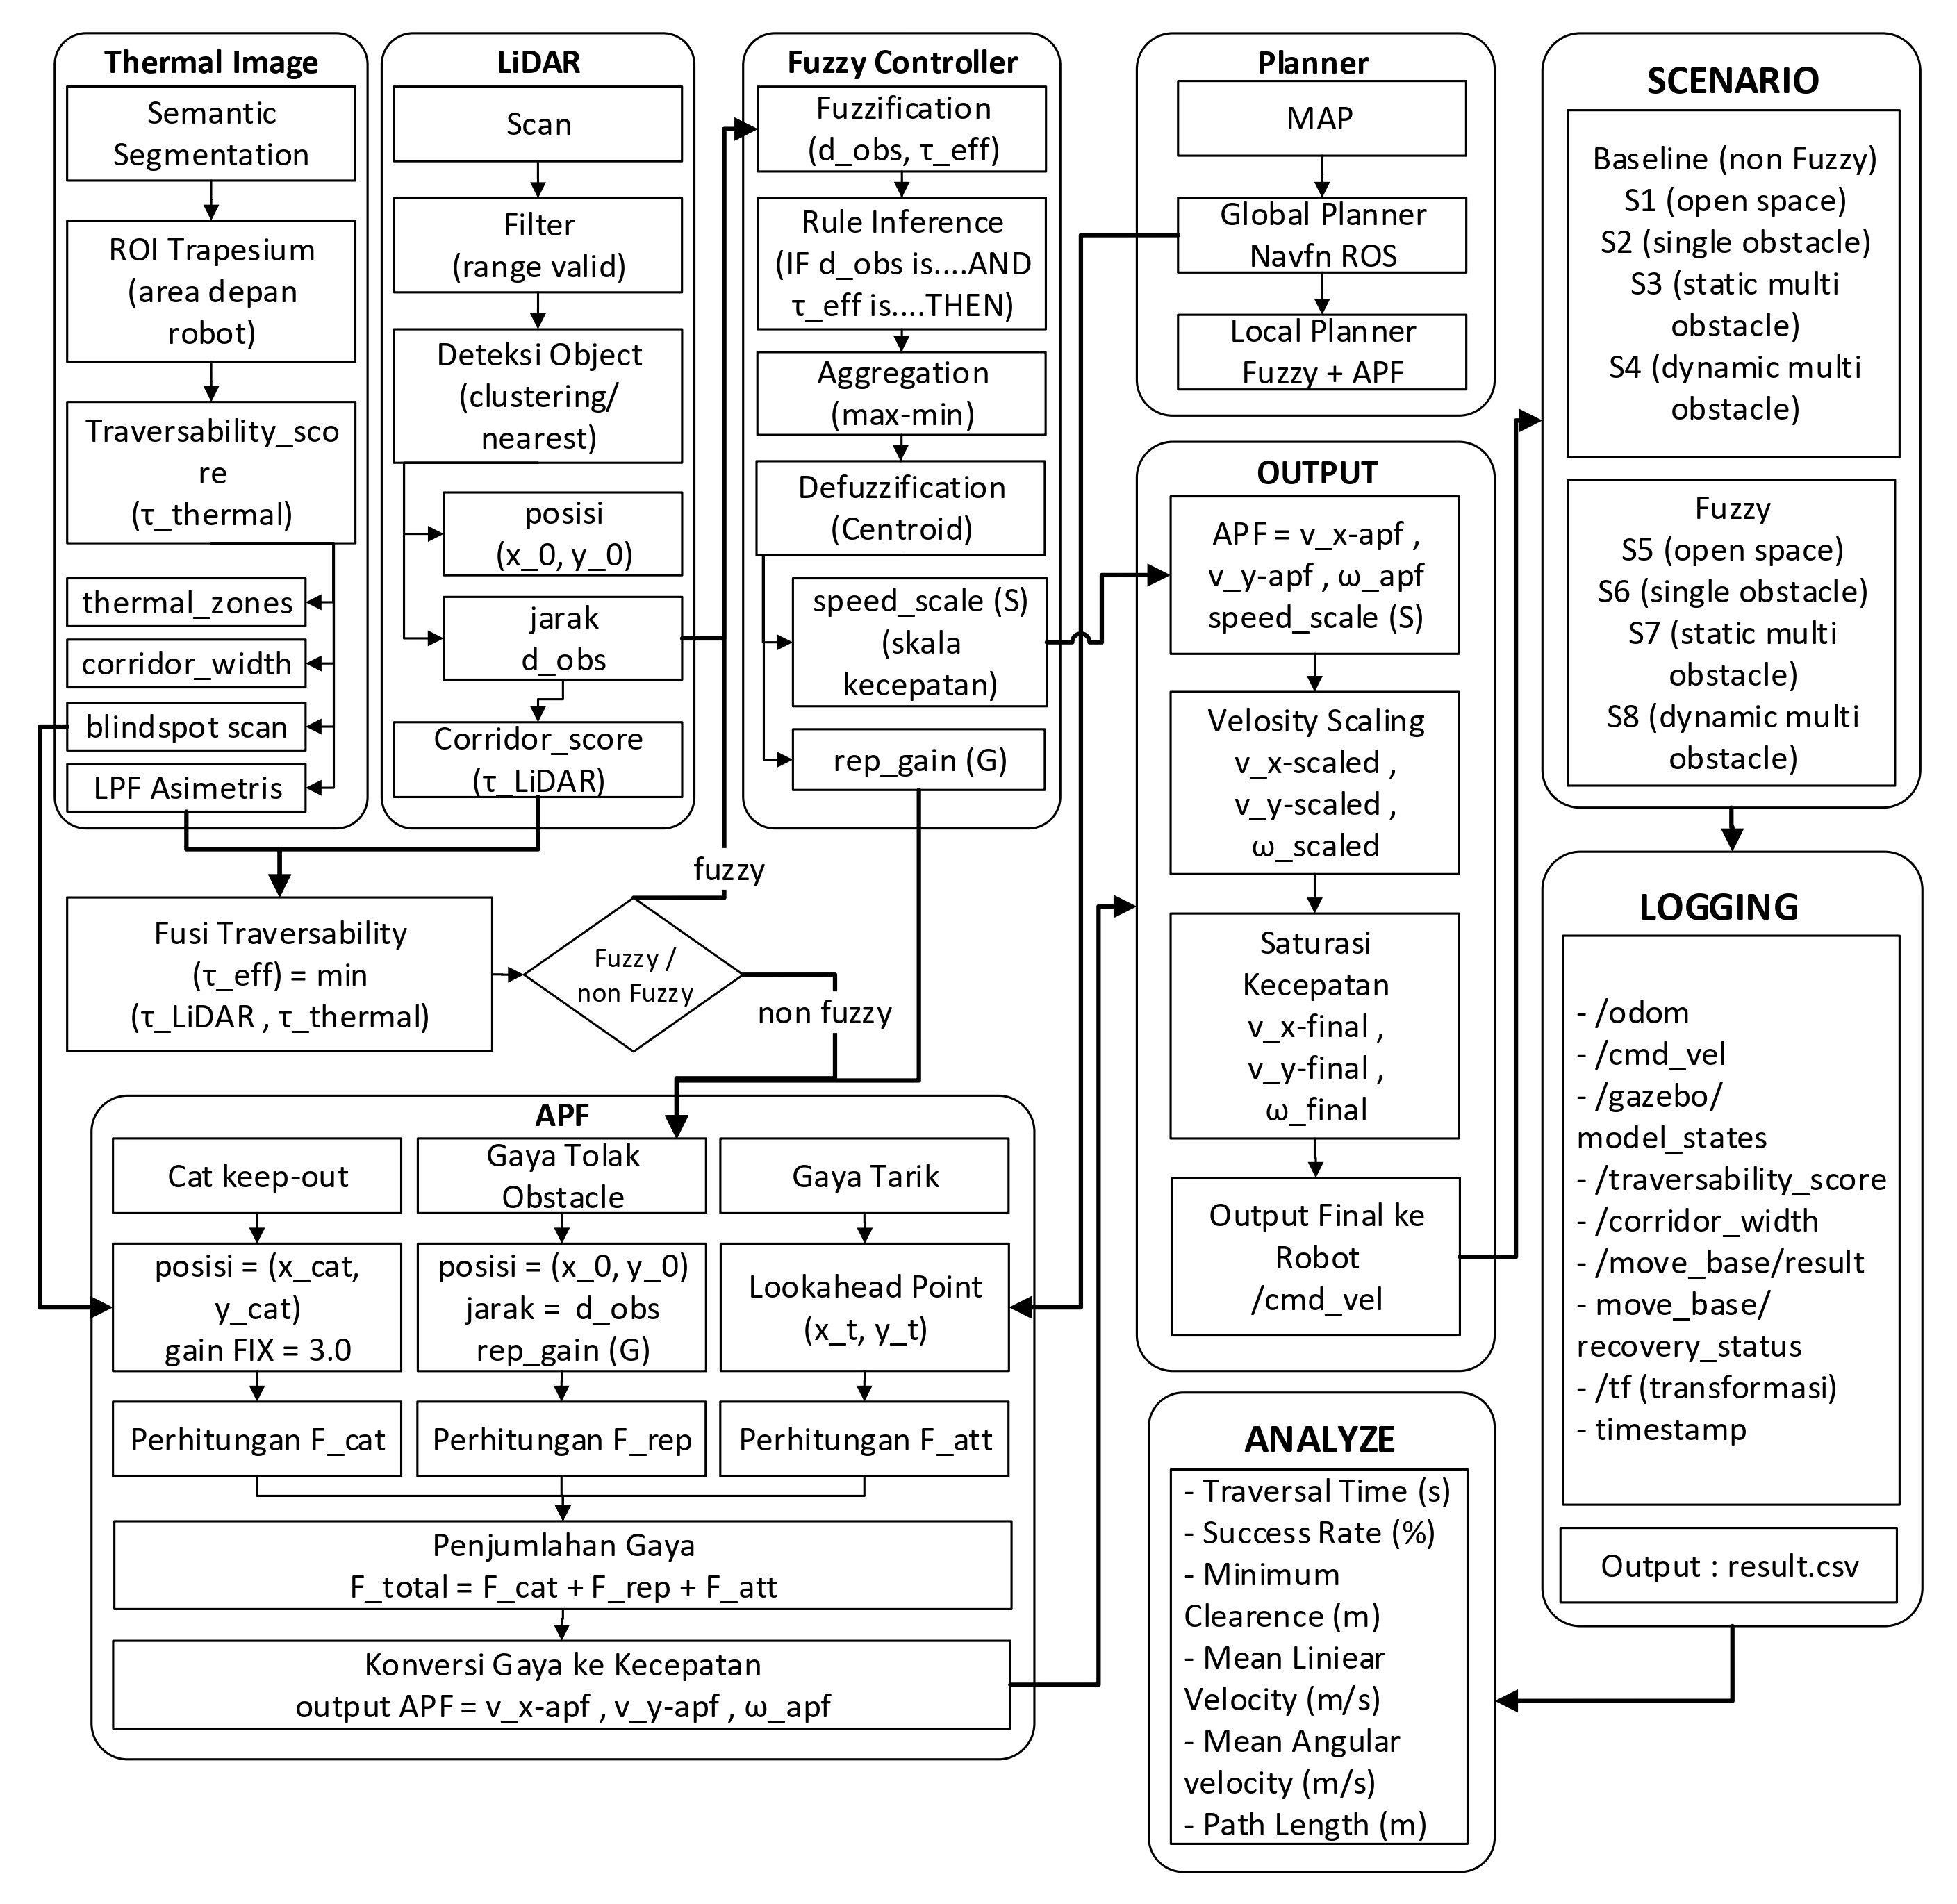
\includegraphics[width=0.92\textwidth]{gambar/3.3_arsitektur_pipeline.jpg}
\caption{Arsitektur sistem navigasi yang diusulkan. Jalur kamera termal (kiri atas) dan jalur LiDAR (kiri bawah) menghasilkan skor \textit{traversability} yang difusikan menjadi \textit{effective traversability}, kemudian diproses oleh pengendali fuzzy Mamdani (tengah) untuk menyesuaikan parameter APF sebelum dipublikasikan sebagai perintah kecepatan robot.}
\label{fig:arsitektur}
\end{figure*}
\FloatBarrier

Untuk mengevaluasi kontribusi pengendali fuzzy, digunakan dua konfigurasi pengujian: \textit{baseline} dan fuzzy. Pada kedua konfigurasi, LiDAR, kamera termal, \textit{virtual scan}, dan fusi \textit{traversability} tetap aktif sehingga informasi lingkungan yang tersedia identik; perbedaan utama hanya terletak pada aktif tidaknya pengendali fuzzy Mamdani pada APFPlanner. Dengan demikian, perbedaan performa yang teramati murni berasal dari mekanisme pengambilan keputusan, bukan dari perbedaan ketersediaan data sensor.

\subsection{Akuisisi dan Pemrosesan Data Sensor}

Pengujian dilaksanakan pada robot beroda tiga \textit{omnidirectional} \texttt{CAD\_ASR\_WITH\_OMNI} dengan \textit{footprint} $0{,}54\times0{,}64$~m, disimulasikan pada ROS Noetic dan Gazebo 11. Sensor LiDAR menghasilkan data \texttt{sensor\_msgs/LaserScan} pada topik \texttt{/scan} dengan cakupan $360^\circ$, frekuensi 40~Hz, dan 720 sampel per siklus. Data ini digunakan untuk mendeteksi jarak \textit{obstacle} terdekat $d_{obs}=\min(D)$ serta mengestimasi \textit{traversability} berbasis lebar koridor bebas $w_{corridor}=d_{left}+d_{right}$, yang dinormalisasi menjadi

\begin{equation}
\tau_{LiDAR}=\mathrm{clip}\!\left(\frac{w_{corridor}-w_{robot}}{w_{ref}},\,0,\,1\right)
\label{eq:trav_lidar}
\end{equation}

Kamera termal dimodelkan melalui \textit{plugin} Gazebo \texttt{libgazebo\_ros\_thermal\_camera}, menghasilkan citra \textit{grayscale} 8-bit beresolusi $640\times480$ piksel pada 10~Hz dengan FOV $90^\circ$ melalui topik \texttt{/thermal/thermal\_camera/image\_raw}. Citra terlebih dahulu melalui koreksi ROI, penajaman, lalu disegmentasi berbasis ambang intensitas menjadi tiga kelas: lantai dapat dilalui (intensitas 45--72), \textit{obstacle} termal (73--255), dan objek dingin/statis (0--44), dilanjutkan operasi morfologi \textit{closing}--\textit{opening} untuk mengurangi \textit{noise} \cite{Castro2016}. Dari citra semantik tersebut diekstraksi skor \textit{traversability} termal berbasis ROI trapesium, lebar koridor, serta kondisi tiga zona navigasi (kiri, tengah, kanan) yang menggambarkan distribusi \textit{obstacle} secara lateral \cite{Sevastopoulos2022}.

\subsection{Fusi LiDAR dan Kamera Termal}
\label{sec:fusi}

\textit{Obstacle} termal yang berada pada area \textit{blind-spot} LiDAR diproyeksikan menjadi \textit{Virtual LaserScan} sejumlah 61 \textit{beam} pada rentang $\theta\in[-0{,}70,\,0{,}70]$~rad ($\pm 40^\circ$) dan dipublikasikan pada topik \texttt{/thermal\_blindspot\_scan} dengan format identik LiDAR. \textit{Virtual scan} ini dimasukkan sebagai lapisan \textit{obstacle} tambahan pada \textit{global costmap} bersama \texttt{/scan}, sehingga \textit{global planner} sudah menghasilkan jalur yang menghindari area \textit{obstacle} termal sejak tahap perencanaan, meskipun objek tidak terlihat LiDAR \cite{Fagundes2024}.

Sebelum difusikan, skor \textit{traversability} termal terlebih dahulu disaring menggunakan \textit{low-pass filter} asimetris dengan koefisien $\alpha=0{,}50$ saat nilai menurun (respons cepat terhadap bahaya) dan $\alpha=0{,}20$ saat nilai naik (mencegah pelepasan keputusan konservatif secara prematur). Nilai \textit{effective traversability} kemudian dihitung menggunakan operator minimum:

\begin{equation}
\tau_{eff}=\min\!\left(\tau_{LiDAR},\,\hat{\tau}_{thermal}\right)
\label{eq:trav_eff}
\end{equation}

Pendekatan ini menerapkan prinsip \textit{safety-first fusion}: apabila salah satu sensor mendeteksi kondisi yang tidak aman, $\tau_{eff}$ akan menurun sehingga robot merespons secara lebih konservatif \cite{Haider2022,Schichler2025}, sebagaimana tergambar pada jalur fusi di tengah Gambar~\ref{fig:arsitektur}.

\subsection{Perancangan Pengendali Fuzzy}

Pengendali fuzzy Mamdani \cite{Mamdani1974} menerima dua masukan, yaitu jarak \textit{obstacle} terdekat $d_{obs}$ (domain $[0{,}0,\,2{,}0]$~m) dan \textit{effective traversability} $\tau_{eff}$ (domain $[0,1]$), masing-masing direpresentasikan dengan tiga label linguistik (Dekat/Sedang/Jauh dan Rendah/Sedang/Tinggi) menggunakan fungsi keanggotaan trapesium pada label ujung dan segitiga pada label tengah. Keluaran berupa \textit{speed scale} $S\in[0,1]$ dan \textit{repulsive gain} $G\in[0{,}5,\,2{,}5]$, juga dengan tiga label (Lambat/Sedang/Cepat dan Lemah/Sedang/Kuat).

Hubungan kedua masukan dan keluaran direpresentasikan melalui sembilan aturan \textit{if-then} sebagaimana dirangkum pada Tabel~\ref{tab:rule_base}: secara umum, robot diperlambat dan gaya tolak diperbesar ketika \textit{obstacle} semakin dekat atau \textit{traversability} menurun.

\begin{table}[!htb]
\centering
\caption{Basis aturan fuzzy Mamdani (Kecepatan, Gain).}
\label{tab:rule_base}
\footnotesize
\begin{tabular}{lccc}
\toprule
\multirow{2}{*}{$d_{obs}$} & \multicolumn{3}{c}{$\tau_{eff}$} \\
\cmidrule(lr){2-4}
 & Rendah & Sedang & Tinggi \\
\midrule
Dekat  & Lambat, Kuat & Lambat, Kuat & Sedang, Kuat \\
Sedang & Lambat, Kuat & Sedang, Sedang & Cepat, Sedang \\
Jauh   & Sedang, Sedang & Cepat, Lemah & Cepat, Lemah \\
\bottomrule
\end{tabular}
\end{table}

Kekuatan aktivasi setiap aturan dihitung dengan operator \textit{AND} minimum, $w_k=\min(\mu_A(d_{obs}),\mu_B(\tau_{eff}))$, seluruh keluaran diagregasi dengan operator maksimum, dan nilai \textit{crisp} akhir diperoleh melalui defuzzifikasi \textit{Center of Gravity}:

\begin{equation}
y^{*}=\frac{\int y\,\mu_{agg}(y)\,dy}{\int \mu_{agg}(y)\,dy}
\label{eq:cog}
\end{equation}

Nilai $S$ dan $G$ yang dihasilkan kemudian memodifikasi parameter APF secara langsung melalui $v=S\cdot v_{base}$ dan $F_{rep}=G\cdot F_{rep}^{base}$, sehingga robot bergerak lebih cepat pada kondisi aman dan secara otomatis memperlambat diri serta memperkuat penghindaran ketika risiko lingkungan meningkat.

\subsection{Sistem Navigasi Robot}

Perencanaan jalur global dilakukan oleh \texttt{NavfnROS} menggunakan algoritma Dijkstra pada \textit{global costmap} yang menggabungkan peta statis (\texttt{grit\_1\_edited\_2}, resolusi 0,05~m/sel) dengan lapisan \textit{obstacle} dari \texttt{/scan} dan \texttt{/thermal\_blindspot\_scan}. Frekuensi \textit{replanning} ditetapkan 0,2~Hz (bukan \textit{default} 1,0~Hz) agar jalur global tidak bergetar akibat pembaruan \textit{virtual scan} termal yang relatif statis dalam jangka pendek.

\textit{Local planner} APFPlanner diimplementasikan sebagai \textit{plugin} \texttt{nav\_core::BaseLocalPlanner} yang berjalan pada 10~Hz, menjumlahkan gaya atraktif menuju \textit{lookahead point} ($d_\text{look}=0{,}7$~m, $k_\text{att}=1{,}5$), gaya repulsif model Khatib \cite{Khatib1986} terhadap \textit{obstacle} LiDAR terdekat ($d_0=0{,}85$~m, diperluas menjadi 1,20~m pada skenario dinamis), dan gaya \textit{cat keep-out} sebagai lapisan keamanan khusus untuk \textit{obstacle} blind-spot:

\begin{equation}
\mathbf{F}_\text{total}=\mathbf{F}_\text{att}+\mathbf{F}_\text{rep}+\mathbf{F}_\text{cat}
\label{eq:f_total}
\end{equation}

Mekanisme \textit{cat keep-out} mengunci posisi \textit{obstacle} blind-spot begitu terdeteksi \textit{virtual scan} termal (mekanisme \textit{latch}) dan mempertahankan jarak aman pusat-ke-pusat $D_\text{safe}=0{,}535$~m dengan zona pengaruh $d_{0c}=0{,}715$~m, sehingga margin keselamatan tetap terjaga meski objek sempat hilang dari sudut pandang kamera. Sistem juga mendeteksi osilasi gaya antar-siklus; apabila arah gaya berbalik tajam (kosinus sudut $<-0{,}5$), \textit{planner} beralih ke mode \textit{AVOIDANCE} sementara untuk memilih arah manuver berdasarkan zona termal yang lebih lapang. Kecepatan akhir dibatasi $v_\text{max}=0{,}2$~m/s dan, pada konfigurasi fuzzy, diskalakan lebih lanjut oleh \textit{speed scale} keluaran fuzzy. Lokalisasi robot diperoleh melalui \texttt{fake\_localization} sehingga evaluasi terfokus pada performa navigasi tanpa dipengaruhi ketidakpastian estimasi posisi.

\section{HASIL DAN PEMBAHASAN}

\subsection{Skenario Pengujian}

Evaluasi dilakukan pada delapan skenario yang dibagi menjadi kelompok \textit{baseline} (S1--S4) dan fuzzy (S5--S8), dengan kondisi lingkungan yang identik pada setiap pasangan (Tabel~\ref{tab:skenario}). Posisi awal dan tujuan ditetapkan sama pada seluruh skenario (START $=(0,0)$, GOAL $=(9{,}159;\,6{,}240)$~m), dan setiap skenario dieksekusi sebanyak sepuluh kali percobaan independen. Seluruh data --- odometri, \texttt{/cmd\_vel}, \textit{traversability}, jarak \textit{obstacle}, status pencapaian tujuan, hingga waktu eksperimen --- dicatat otomatis oleh \texttt{experiment\_logger.py} dan disimpan dalam berkas CSV untuk dianalisis secara statistik menggunakan uji non-parametrik Mann--Whitney $U$ ($\alpha=0{,}05$) karena ukuran sampel per kelompok relatif kecil ($n=10$) \cite{Adiuku2024}.

\begin{table}[!htb]
\centering
\caption{Skenario pengujian yang digunakan.}
\label{tab:skenario}
\footnotesize
\begin{tabular}{cccc}
\toprule
Skenario & Konfig. & Kondisi Lingkungan & Fuzzy \\
\midrule
S1 & \textit{Baseline} & Tanpa \textit{obstacle} & Tidak \\
S2 & \textit{Baseline} & Satu \textit{obstacle} manusia & Tidak \\
S3 & \textit{Baseline} & Majemuk statis + kucing & Tidak \\
S4 & \textit{Baseline} & Majemuk dinamis + kucing & Tidak \\
S5 & Fuzzy & Tanpa \textit{obstacle} & Ya \\
S6 & Fuzzy & Satu \textit{obstacle} manusia & Ya \\
S7 & Fuzzy & Majemuk statis + kucing & Ya \\
S8 & Fuzzy & Majemuk dinamis + kucing & Ya \\
\bottomrule
\end{tabular}
\end{table}

\textit{Obstacle} ``kucing'' (\texttt{obstacle\_cat}, $r=0{,}18$~m, tinggi $\approx0{,}19$~m) sengaja ditempatkan pada area \textit{blind-spot} LiDAR untuk menguji hipotesis utama penelitian, sedangkan skenario S4/S8 menambahkan dua \textit{obstacle} manusia yang bergerak osilasi dengan kecepatan puncak hingga $\approx0{,}81$~m/s untuk merepresentasikan kondisi dinamis.

\subsection{Analisis Kinerja Sistem}

Tabel~\ref{tab:hasil} merangkum \textit{Success Rate} (SR), \textit{Collision-Free Rate} (CFR), dan rata-rata \textit{minimum clearance} ($c_{min}$) pada seluruh skenario. Pada lingkungan sederhana (S1/S5 dan S2/S6), kedua konfigurasi sama-sama mencapai SR dan CFR 100\%, dengan peningkatan $c_{min}$ yang relatif kecil (dari $0{,}4301$ menjadi $0{,}4370$~m) karena \textit{obstacle} manusia sudah terdeteksi penuh oleh LiDAR.

\begin{table}[!htb]
\centering
\caption{Ringkasan hasil pengujian seluruh skenario.}
\label{tab:hasil}
\footnotesize
\begin{tabular}{ccccc}
\toprule
Skenario & Konfig. & SR (\%) & CFR (\%) & $c_{min}$ (m) \\
\midrule
S1 & \textit{Baseline} & 100 & 100 & 0,0000 \\
S2 & \textit{Baseline} & 100 & 100 & 0,4301 \\
S3 & \textit{Baseline} & 65 & 65 & 0,0346 \\
S4 & \textit{Baseline} & 0 & 0 & $-0{,}1635$ \\
S5 & Fuzzy & 100 & 100 & 0,0000 \\
S6 & Fuzzy & 100 & 100 & 0,4370 \\
S7 & Fuzzy & 100 & 100 & 0,1825 \\
S8 & Fuzzy & 100 & 100 & 0,3167 \\
\bottomrule
\end{tabular}
\end{table}

Perbedaan signifikan muncul pada lingkungan kompleks. Pada S3, konfigurasi \textit{baseline} hanya berhasil pada 65\% percobaan dengan $c_{min}$ rata-rata sebesar $0{,}0346$~m, yang berarti robot bergerak sangat dekat dengan \textit{obstacle} blind-spot. Setelah fuzzy diaktifkan (S7), SR dan CFR naik menjadi 100\% dan $c_{min}$ meningkat lebih dari lima kali lipat menjadi $0{,}1825$~m. Perbedaan paling ekstrem terlihat pada pasangan S4--S8: seluruh percobaan \textit{baseline} pada S4 mengalami tabrakan ($c_{min}=-0{,}1635$~m, SR/CFR $=0\%$), sedangkan seluruh percobaan fuzzy pada S8 berhasil dengan $c_{min}$ positif sebesar $0{,}3167$~m. Gambar~\ref{fig:traj} memvisualisasikan kontras tersebut: lintasan S4 secara konsisten menabrak \textit{obstacle} kucing yang tidak terdeteksi LiDAR, sedangkan lintasan S8 menyusur dengan margin aman pada sisi yang sama.

\begin{figure}[H]
\centering
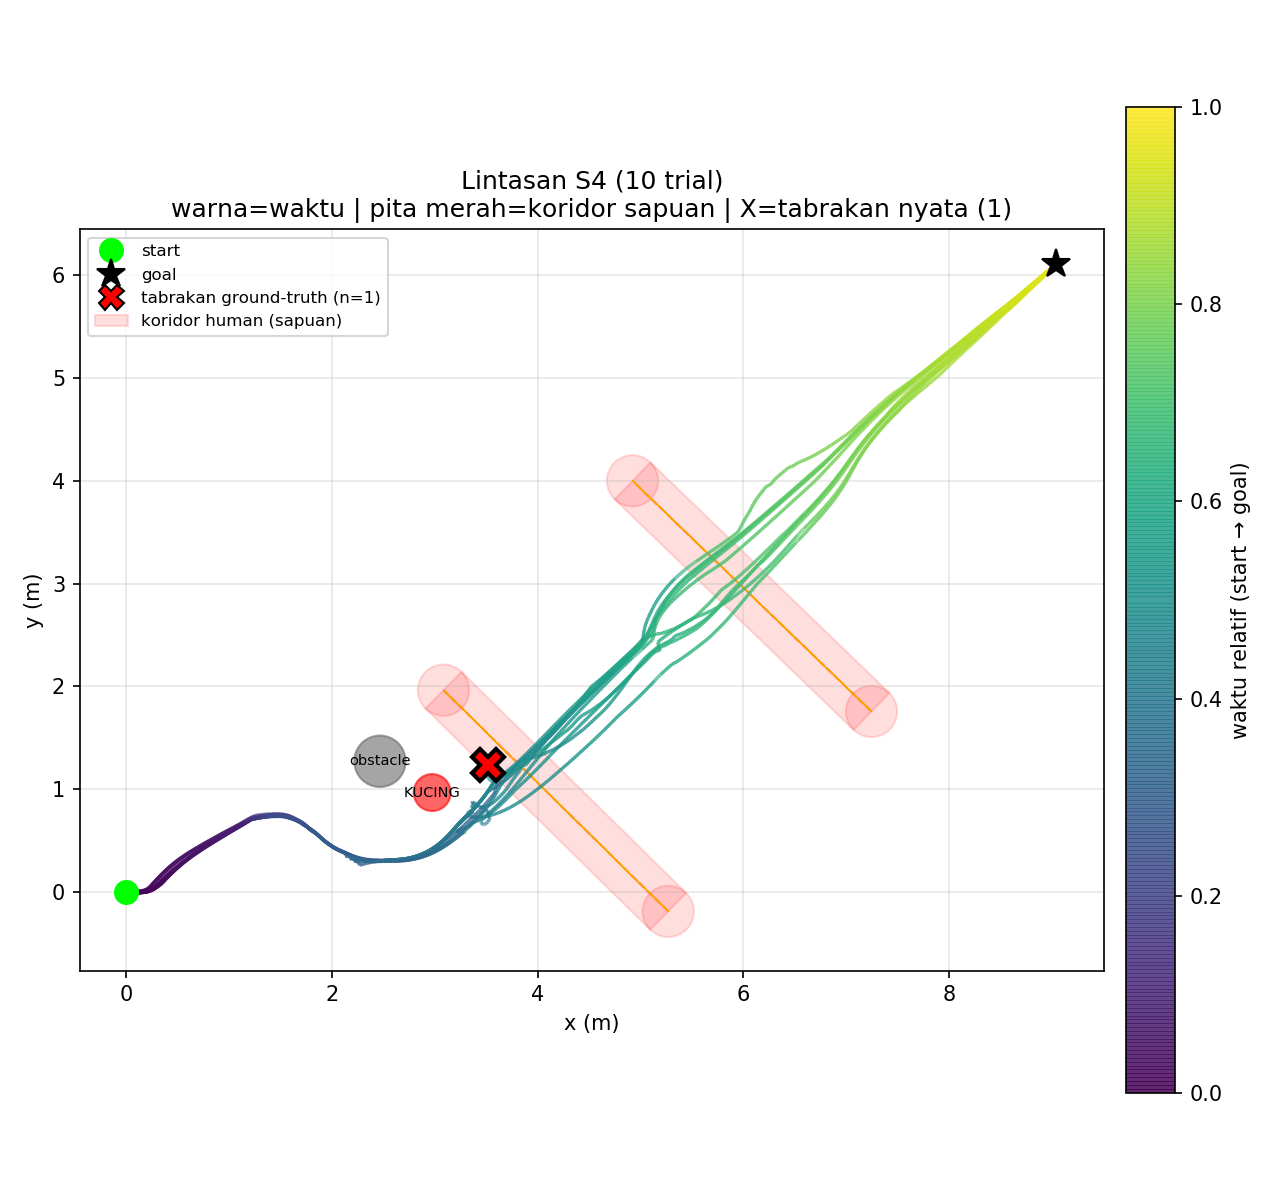
\includegraphics[width=0.7\linewidth]{gambar/4.6_traj_S4_dynamic.png}
\vspace{0.5em}
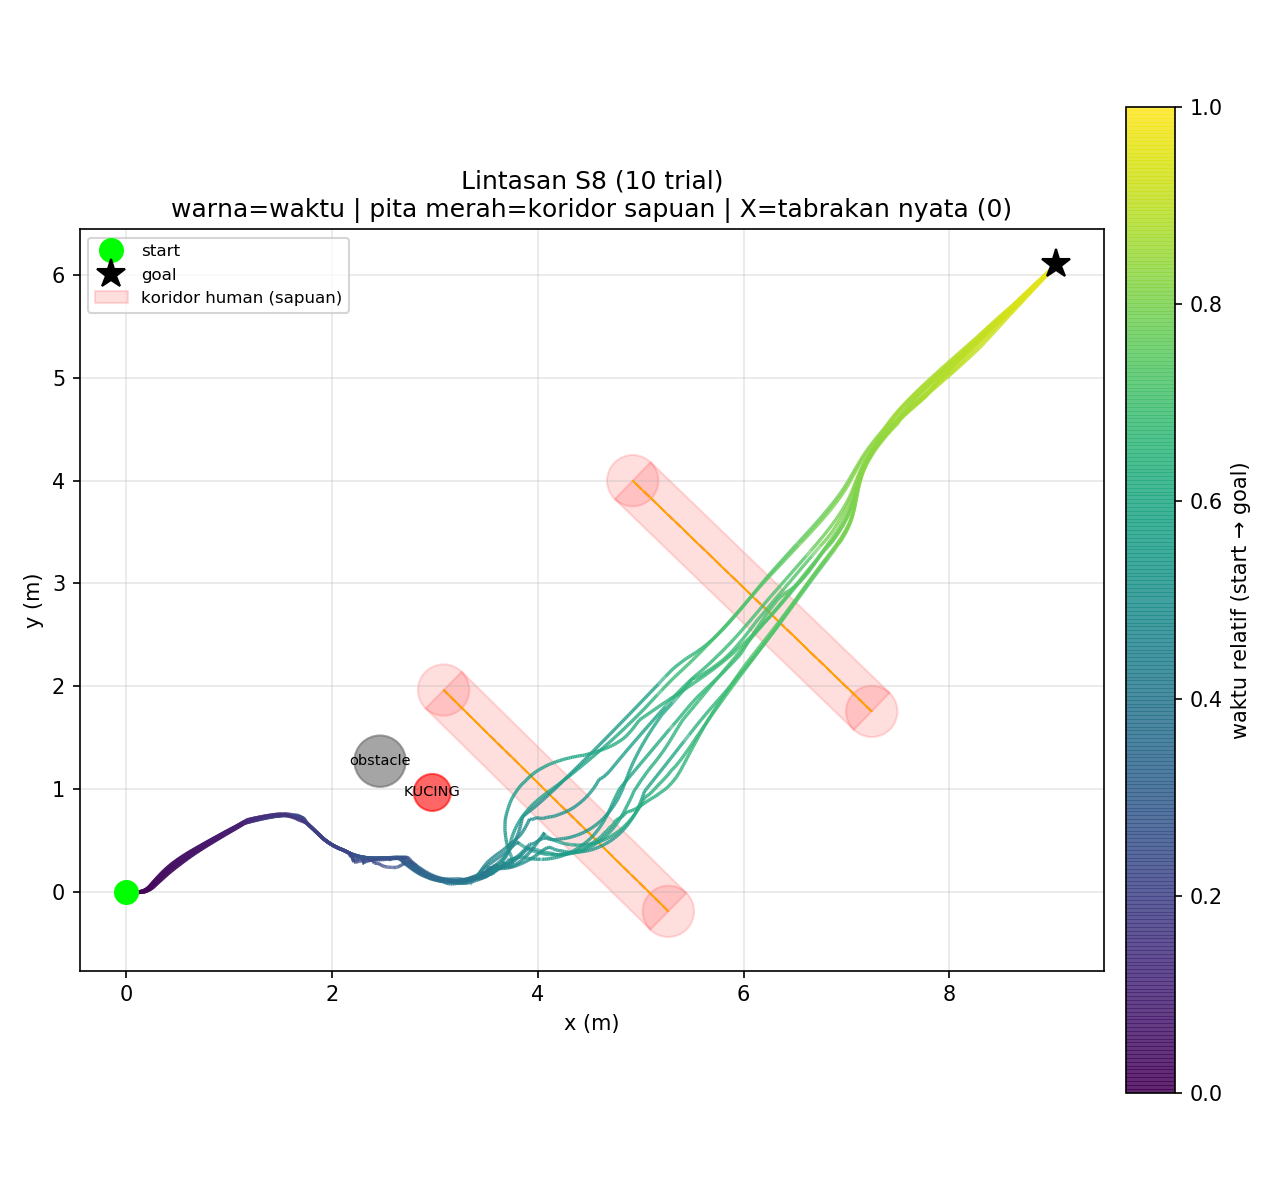
\includegraphics[width=0.7\linewidth]{gambar/4.6_traj_S8_dynamic.png}
\caption{Perbandingan lintasan pada skenario \textit{obstacle} dinamis (10 \textit{trial}). Atas: konfigurasi \textit{baseline} (S4) --- seluruh lintasan menabrak \textit{obstacle} kucing (tanda X) yang berada pada \textit{blind-spot} LiDAR. Bawah: konfigurasi fuzzy (S8) --- seluruh lintasan berhasil menyusur melewati \textit{obstacle} dengan margin aman tanpa tabrakan.}
\label{fig:traj}
\end{figure}

Uji Mann--Whitney $U$ terhadap $c_{min}$ menunjukkan bahwa peningkatan tersebut signifikan secara statistik: $p=0{,}0013$ dengan \textit{effect size} $r=0{,}80$ (besar) pada S2--S6, serta $p<0{,}001$ dengan $r=1{,}00$ (sangat besar) pada S3--S7 dan S4--S8 \cite{Kerby2014}. Gambar~\ref{fig:boxplot} menunjukkan bahwa konfigurasi fuzzy tidak hanya menaikkan nilai rata-rata, tetapi menggeser seluruh distribusi $c_{min}$ menuju nilai yang lebih aman, sekaligus menghilangkan kejadian tabrakan yang muncul pada \textit{baseline}.

\begin{figure}[H]
\centering
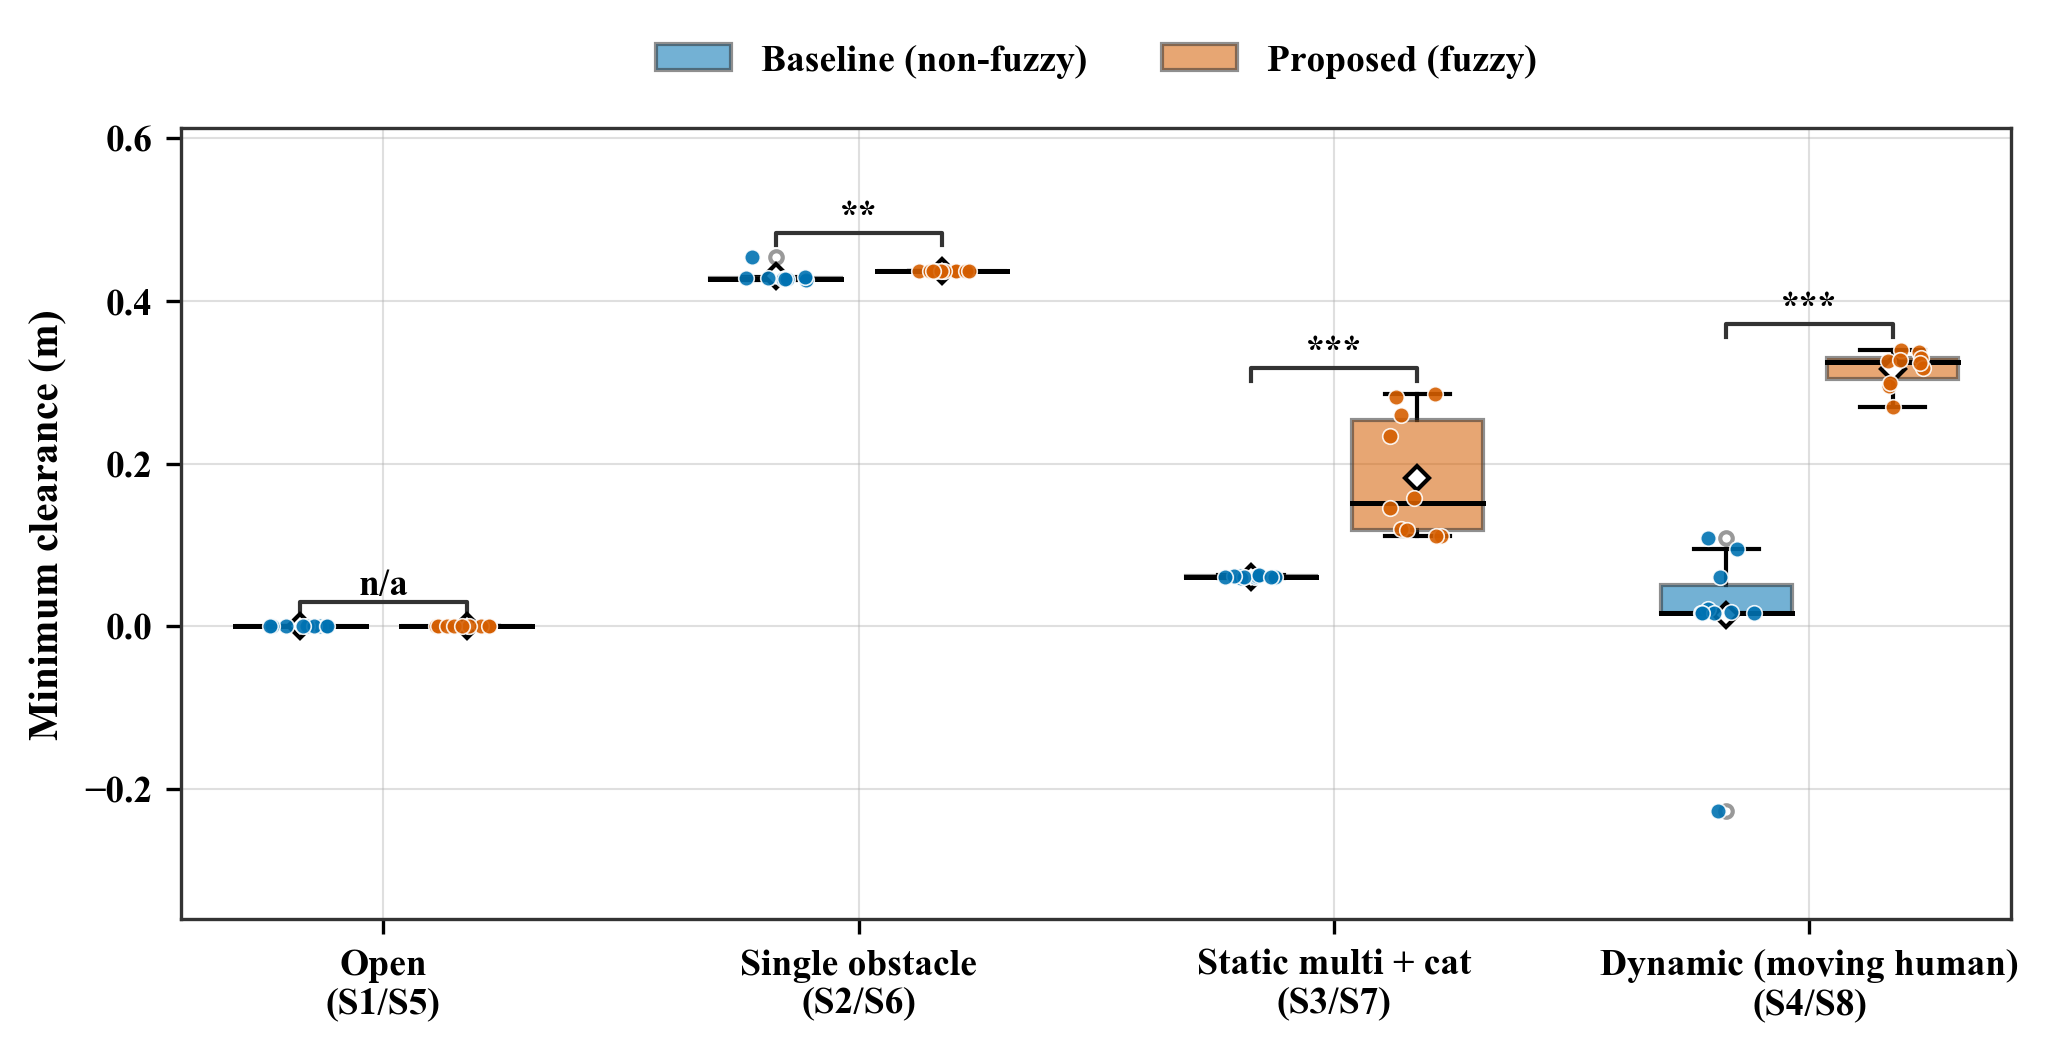
\includegraphics[width=0.45\textwidth]{gambar/4.4_clearance_boxplot.png}
\caption{Distribusi \textit{minimum clearance} pada keempat pasangan skenario. Tanda bintang menunjukkan signifikansi uji Mann--Whitney $U$ (** $p<0{,}01$; *** $p<0{,}001$); n/a menandakan kedua kelompok tidak berbeda (lingkungan tanpa \textit{obstacle}).}
\label{fig:boxplot}
\end{figure}
\FloatBarrier

\subsection{Pengaruh Deteksi Blind-Spot LiDAR}

Salah satu tujuan utama penelitian ini adalah mengatasi keterbatasan LiDAR 2D terhadap \textit{obstacle} berprofil rendah yang berada di luar bidang pemindaian sensor. Keterbatasan tersebut terlihat jelas pada skenario S3 dan S4 yang mengandung \textit{obstacle} kucing pada area \textit{blind-spot} LiDAR. Pada konfigurasi \textit{baseline}, keberadaan \textit{obstacle} tersebut menyebabkan penurunan performa navigasi yang signifikan. Nilai \textit{Success Rate} dan \textit{Collision-Free Rate} pada S3 hanya mencapai 65\%, sedangkan seluruh percobaan pada S4 mengalami kegagalan akibat tabrakan.

Integrasi kamera termal memungkinkan \textit{obstacle} yang tidak terdeteksi LiDAR direpresentasikan melalui mekanisme \textit{Virtual LaserScan} dan ditambahkan ke dalam \textit{global costmap}. Dengan demikian, \textit{global planner} maupun \textit{local planner} memperoleh informasi tambahan mengenai keberadaan area berbahaya yang sebelumnya tidak tersedia pada konfigurasi \textit{baseline}.

Hasil pengujian menunjukkan bahwa aktivasi mekanisme tersebut, yang dikombinasikan dengan pengendali fuzzy Mamdani, meningkatkan SR dan CFR menjadi 100\% pada S7 dan S8. Selain itu, nilai \textit{minimum clearance} meningkat dari 0,0346~m menjadi 0,1825~m pada pasangan S3--S7 dan dari $-0,1635$~m menjadi 0,3167~m pada pasangan S4--S8. Hasil tersebut menunjukkan bahwa metode yang diusulkan tidak hanya meningkatkan kemampuan deteksi \textit{obstacle}, tetapi juga meningkatkan margin keselamatan navigasi ketika robot beroperasi pada lingkungan yang mengandung area \textit{blind-spot} LiDAR.

Peningkatan keselamatan tersebut disertai \textit{trade-off} pada efisiensi temporal: median waktu tempuh pada lingkungan terbuka meningkat dari $\approx25{,}5$~s (S1) menjadi $\approx31$~s (S5), dan peningkatan yang lebih besar terjadi pada S7 dan S8 karena robot memperlambat diri lebih awal saat mendekati \textit{obstacle}. Sebaliknya, panjang lintasan hanya bertambah relatif kecil karena robot tetap mengikuti jalur global yang sama dan hanya menyesuaikan manuver lokal. Menariknya, kecepatan angular rata-rata pada konfigurasi fuzzy justru cenderung lebih rendah dan lebih stabil dibandingkan \textit{baseline}, karena manuver penghindaran dimulai lebih awal dan bersifat gradual, bukan koreksi arah mendadak.

\subsection{Peran Mekanisme Cat Keep-Out}

Selain kontribusi kamera termal dan pengendali fuzzy, peningkatan performa pada skenario yang mengandung \textit{obstacle} berprofil rendah juga dipengaruhi oleh mekanisme \textit{cat keep-out} yang diintegrasikan pada APFPlanner. Mekanisme ini dirancang khusus untuk mempertahankan representasi \textit{obstacle} blind-spot setelah pertama kali terdeteksi oleh kamera termal, sehingga robot tidak langsung menganggap area tersebut aman ketika \textit{obstacle} sementara keluar dari bidang pandang sensor.

Pada konfigurasi \textit{baseline}, keputusan navigasi sepenuhnya bergantung pada kondisi persepsi saat itu (\textit{instantaneous perception}). Akibatnya, \textit{obstacle} yang tidak teramati LiDAR berpotensi menyebabkan robot kembali bergerak menuju area berbahaya. Sebaliknya, mekanisme \textit{cat keep-out} mempertahankan zona penghindaran selama periode tertentu sehingga robot tetap menjaga jarak aman terhadap \textit{obstacle} yang sebelumnya telah terdeteksi.

Kombinasi antara \textit{virtual scan}, fusi \textit{traversability}, pengendali fuzzy, dan \textit{cat keep-out} menghasilkan lapisan keselamatan berjenjang yang saling melengkapi. Pendekatan tersebut memungkinkan robot tidak hanya mendeteksi \textit{obstacle} blind-spot, tetapi juga mempertahankan keputusan penghindaran secara konsisten hingga risiko tabrakan benar-benar berkurang.

\subsection{Pembahasan Hasil}

Temuan ini menunjukkan bahwa kontribusi kamera termal dan dua mekanismenya --- \textit{virtual scan} pada \textit{global costmap} dan fusi \textit{traversability} \eqref{eq:trav_eff} pada lapisan kendali lokal --- saling melengkapi. \textit{Virtual scan} membuat \textit{global planner} ``sadar'' terhadap \textit{obstacle} blind-spot sejak tahap perencanaan jalur, sementara fusi \textit{traversability} dan pengendali fuzzy menentukan seberapa hati-hati robot bergerak ketika benar-benar mendekati area berisiko. Prinsip \textit{safety-first fusion} (operator minimum pada Persamaan~\ref{eq:trav_eff}) memastikan bahwa sumber bahaya mana pun --- baik koridor LiDAR yang sempit maupun area termal yang terhalang panas --- akan menurunkan $\tau_{eff}$ dan memicu respons konservatif, tanpa memerlukan perubahan struktur dasar ROS Navigation Stack.

Hasil juga memperlihatkan bahwa peningkatan keselamatan paling signifikan justru terjadi pada skenario yang sebelumnya menjadi kelemahan utama LiDAR 2D, yaitu \textit{obstacle} berprofil rendah dan \textit{obstacle} dinamis, sedangkan pada skenario sederhana dengan \textit{obstacle} yang sudah sepenuhnya teramati LiDAR, kontribusi tambahan fuzzy relatif kecil. Pola ini konsisten dengan tujuan perancangan sistem, yaitu melengkapi --- bukan menggantikan --- kemampuan deteksi LiDAR.

\textit{Trade-off} berupa penambahan waktu tempuh dan panjang lintasan tergolong wajar mengingat besarnya peningkatan margin keselamatan yang diperoleh, terutama pada skenario yang sebelumnya menghasilkan tabrakan total (S4). Penelitian ini masih dibatasi pada lingkungan simulasi dengan lokalisasi \textit{ground-truth} (\texttt{fake\_localization}) dan satu peta \textit{indoor}, sehingga validasi pada robot fisik dengan ketidakpastian sensor dan lokalisasi nyata menjadi langkah lanjutan yang penting.

\subsection{Implikasi terhadap Implementasi Robot Nyata}

Meskipun penelitian ini dilakukan pada lingkungan simulasi, hasil yang diperoleh menunjukkan bahwa pendekatan yang diusulkan memiliki potensi untuk diterapkan pada robot bergerak nyata dengan kebutuhan komputasi yang relatif rendah. Seluruh proses pengambilan keputusan dilakukan menggunakan logika fuzzy Mamdani dan operasi fusi sederhana berbasis \textit{minimum operator}, sehingga tidak memerlukan sumber daya komputasi sebesar metode berbasis \textit{deep learning}.

Karakteristik tersebut menjadikan metode yang diusulkan sesuai untuk platform robot bergerak berbiaya rendah maupun sistem berbasis komputasi tepi (\textit{edge computing}) yang memiliki keterbatasan sumber daya. Selain itu, karena implementasi dilakukan di atas ROS Navigation Stack tanpa mengubah struktur dasarnya, metode ini dapat diintegrasikan pada berbagai platform robot yang telah menggunakan ekosistem ROS secara relatif mudah.

\section{KESIMPULAN}

Berdasarkan hasil perancangan dan pengujian, dapat disimpulkan bahwa integrasi LiDAR 2D dan kamera termal melalui \textit{decision-level fusion} berhasil menghasilkan representasi kondisi lingkungan yang lebih lengkap dibandingkan penggunaan LiDAR saja. Pengendali fuzzy Mamdani yang memanfaatkan jarak \textit{obstacle} dan \textit{effective traversability} mampu menyesuaikan parameter APF secara adaptif sehingga robot dapat merespons perubahan tingkat risiko lingkungan secara lebih aman.

Konfigurasi fuzzy berhasil mempertahankan \textit{Success Rate} dan \textit{Collision-Free Rate} sebesar 100\% pada seluruh skenario pengujian. Pada lingkungan kompleks yang mengandung \textit{obstacle} statis maupun dinamis, nilai \textit{minimum clearance} meningkat dari 0,0346~m menjadi 0,1825~m pada pasangan S3--S7 dan dari $-0,1635$~m menjadi 0,3167~m pada pasangan S4--S8. Hasil tersebut menunjukkan bahwa metode yang diusulkan mampu menghilangkan kegagalan navigasi yang disebabkan oleh \textit{blind-spot} LiDAR tanpa mengubah struktur dasar ROS Navigation Stack.

Sebagai pengembangan lanjutan, penelitian ini dapat diperluas melalui implementasi pada robot fisik, pemanfaatan segmentasi termal berbasis \textit{deep learning}, serta penerapan metode fusi sensor tingkat fitur untuk meningkatkan robustitas sistem pada lingkungan yang lebih kompleks dan dinamis.

\balance
{\footnotesize
\begin{thebibliography}{99}

\bibitem{Liu2024} Y. Liu, S. Wang, Y. Xie, T. Xiong, and M. Wu, ``A Review of Sensing Technologies for Indoor Autonomous Mobile Robots,'' \textit{Sensors}, vol. 24, no. 4, p. 1222, 2024, doi: 10.3390/s24041222.

\bibitem{Macenski2022} S. Macenski, T. Foote, B. Gerkey, C. Lalancette, and W. Woodall, ``Robot Operating System 2: Design, Architecture, and Uses in the Wild,'' \textit{Science Robotics}, vol. 7, no. 66, p. eabm6074, 2022, doi: 10.1126/scirobotics.abm6074.

\bibitem{Fagundes2024} L. A. Fagundes, A. G. Caldeira, M. B. Quemelli, F. N. Martins, and A. S. Brand\~{a}o, ``Analytical Formalism for Data Representation and Object Detection with 2D LiDAR: Application in Mobile Robotics,'' \textit{Sensors}, vol. 24, no. 7, p. 2284, 2024, doi: 10.3390/s24072284.

\bibitem{Kibii2022} J. E. Kibii, A. Dreher, P. L. Wormser, and H. Gimpel, ``Design and Calibration of Plane Mirror Setups for Mobile Robots with a 2D-Lidar,'' \textit{Sensors}, vol. 22, no. 20, p. 7830, 2022, doi: 10.3390/s22207830.

\bibitem{Castro2016} L. E. Castro Jim\'{e}nez and E. A. Mart\'{i}nez-Garc\'{i}a, ``Thermal Image Sensing Model for Robotic Planning and Search,'' \textit{Sensors}, vol. 16, no. 8, p. 1253, 2016, doi: 10.3390/s16081253.

\bibitem{Choi2023} J. D. Choi and M. Y. Kim, ``A Sensor Fusion System with Thermal Infrared Camera and LiDAR for Autonomous Vehicles and Deep Learning Based Object Detection,'' \textit{ICT Express}, vol. 9, no. 2, pp. 222--227, 2023, doi: 10.1016/j.icte.2021.12.016.

\bibitem{Schichler2025} L. Schichler, K. Festl, and S. Solmaz, ``Robust Multi-Sensor Fusion for Localization in Hazardous Environments Using Thermal, LiDAR, and GNSS Data,'' \textit{Sensors}, vol. 25, no. 7, p. 2032, 2025, doi: 10.3390/s25072032.

\bibitem{Khatib1986} O. Khatib, ``Real-Time Obstacle Avoidance for Manipulators and Mobile Robots,'' \textit{The International Journal of Robotics Research}, vol. 5, no. 1, pp. 90--98, 1986, doi: 10.1177/027836498600500106.

\bibitem{Lv2024} Q. Lv, G. Hao, Z. Huang, B. Li, D. Fu, H. Zhao, W. Chen, and S. Chen, ``Localized Path Planning for Mobile Robots Based on a Subarea-Artificial Potential Field Model,'' \textit{Sensors}, vol. 24, no. 11, p. 3604, 2024, doi: 10.3390/s24113604.

\bibitem{Haider2022} M. H. Haider, Z. Wang, A. A. Khan, \textit{et al.}, ``Robust Mobile Robot Navigation in Cluttered Environments Based on Hybrid Adaptive Neuro-Fuzzy Inference and Sensor Fusion,'' \textit{J. King Saud Univ. -- Comput. Inf. Sci.}, vol. 34, no. 10, pp. 9060--9070, 2022, doi: 10.1016/j.jksuci.2022.08.031.

\bibitem{Benaicha2026} Benaicha \textit{et al.}, ``An Improved Fuzzy Logic Controller for Mobile Robots Navigation in Unknown Environments,'' \textit{Journal of Field Robotics}, 2026, doi: 10.1002/rob.70037.

\bibitem{Sevastopoulos2022} C. Sevastopoulos and S. Konstantopoulos, ``A Survey of Traversability Estimation for Mobile Robots,'' \textit{IEEE Access}, vol. 10, pp. 96331--96347, 2022, doi: 10.1109/ACCESS.2022.3202545.

\bibitem{Mamdani1974} E. H. Mamdani, ``Application of Fuzzy Algorithms for Control of Simple Dynamic Plant,'' \textit{Proc. Inst. Electr. Eng.}, vol. 121, no. 12, pp. 1585--1588, 1974, doi: 10.1049/piee.1974.0328.

\bibitem{Adiuku2024} N. Adiuku, N. P. Avdelidis, G. Tang, and A. Plastropoulos, ``Improved Hybrid Model for Obstacle Detection and Avoidance in Robot Operating System Framework (RRT and Dynamic Windows Approach),'' \textit{Sensors}, vol. 24, no. 7, p. 2262, 2024, doi: 10.3390/s24072262.

\bibitem{Kerby2014} D. S. Kerby, ``The Simple Difference Formula: An Approach to Teaching Nonparametric Correlation,'' \textit{Comprehensive Psychology}, vol. 3, p. 11.IT.3.1, 2014, doi: 10.2466/11.IT.3.1.

\end{thebibliography}
}

\section*{Lampiran}

Seluruh kode program, berkas konfigurasi, model simulasi, serta data pendukung yang digunakan dalam penelitian ini tersedia pada repositori GitHub berikut.

\begin{center}
{\footnotesize
\url{https://github.com/PriagungRA/TA-Autonomous-Robot-Navigation-Fuzzy-Lidar-Thermal}
}
\end{center}

Repositori tersebut memuat implementasi lengkap sistem navigasi robot beroda otonom berbasis fusi sensor LiDAR dan kamera termal yang digunakan pada penelitian ini. Seluruh modul dikembangkan pada lingkungan Robot Operating System (ROS) Noetic dan digunakan untuk merealisasikan skenario pengujian yang dilaporkan pada makalah.

Artefak penelitian yang tersedia pada repositori meliputi:

\begin{itemize}
\item Implementasi \textit{Artificial Potential Field Planner} (APFPlanner) sebagai \textit{local planner}.
\item Implementasi pengendali logika fuzzy Mamdani untuk penyesuaian \textit{speed scale} dan \textit{repulsive gain}.
\item Modul fusi traversability LiDAR dan kamera termal berbasis \textit{decision-level fusion}.
\item Implementasi pembentukan \textit{Virtual LaserScan} untuk deteksi obstacle pada area \textit{blind-spot} LiDAR.
\item Berkas konfigurasi ROS Navigation Stack, \textit{costmap}, parameter planner, dan \textit{launch file}.
\item Model robot dan lingkungan simulasi Gazebo yang digunakan pada seluruh skenario eksperimen.
\item Skrip pencatatan data dan pengolahan hasil evaluasi penelitian.
\end{itemize}

Penyediaan repositori penelitian bertujuan untuk meningkatkan transparansi, reproduktibilitas, dan kemudahan pengembangan lebih lanjut terhadap metode yang diusulkan. Seluruh artefak yang diperlukan untuk menjalankan simulasi dan memverifikasi hasil penelitian tersedia secara terbuka pada repositori tersebut.
\end{document}